% <! - - Lý do tiếp theo là một trong những lý do lớn nhất khiến tổ chức cần chuyển đổi nhu cầu và mong đợi của khách hàng liên tục thay đổi để duy trì và mở rộng cơ sở khách hàng của mình. - - >
% <! - - Các tổ chức cần điều chỉnh hoạt động kinh doanh của mình để đáp ứng nhu cầu và mong đợi của khách hàng. Các doanh nghiệp bỏ qua kỳ vọng của khách hàng có xu hướng thua đối thủ cạnh tranh. - - >
% <! - - Vì vậy, điều xảy ra với những doanh nghiệp không chuyển đổi, câu trả lời ngắn gọn cho câu hỏi này là những doanh nghiệp không chuyển đổi sẽ không thể tồn tại. - - >

% <! - - Một điểm quan trọng cần ghi nhớ là chuyển đổi không phải là sáng kiến hay nhiệm vụ chỉ diễn ra một lần. Các doanh nghiệp cần thay đổi liên tục và điều này đòi hỏi những thay đổi nhanh chóng đối với hệ thống và ứng dụng của họ. - - >

% <! - - Một thách thức chung mà các doanh nghiệp phải đối mặt trong hành trình chuyển đổi là cách xây dựng phần mềm cũ cản trở hoặc gây khó khăn cho các tổ chức trong việc chuyển đổi. - - >

Trong quá trình hoạt động, không phải mọi doanh nghiệp đều sẽ giữ nguyên mô hình kinh doanh được đưa ra ban đầu của mình. Khi quy mô thị trường thay đổi thì việc chuyển đổi mô hình kinh doanh là điều cần thiết. Chuyển đổi kinh doanh như một công cụ linh hoạt giúp các doanh nghiệp có thể phát triển và tồn tại giữa các đối thủ của mình.

Ví dụ:
Amazon từ hiệu sách trực tuyến thành thị trường cho nhà cung cấp khác như: Thương mại điện tử (E - commerce), Dịch vụ đám mây (Cloud Computing),...

<! - - !Thêm google - - >

% ![](pictures/KienTrucViDichVuAmazon.png)
% ![](pictures/KienTrucViDichVuAmazon.png)

\begin{figure}[h]
\centering
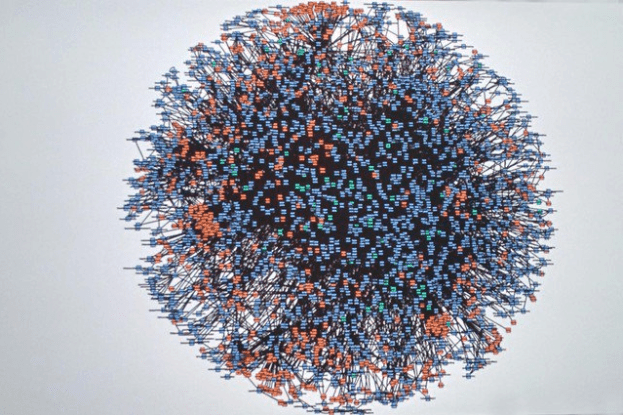
\includegraphics[height = 3cm]{pictures/KienTrucViDichVuAmazon.png}
% \caption{ViDuHinhAnhTheoChieuDoc}
\end{figure}

\begin{figure}[h]
\centering
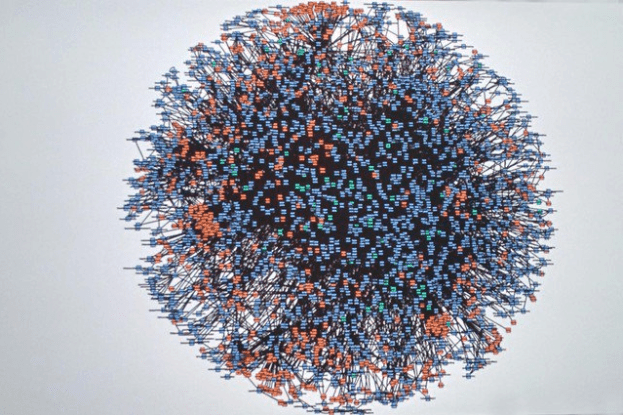
\includegraphics[height = 3cm]{pictures/KienTrucViDichVuAmazon.png}
% \caption{ViDuHinhAnhTheoChieuDoc}
\end{figure}

<! - - Hình kiến trúc vi dịch vụ của Amazon - - >
<! - - !Thêm google - - >

Gần đây, Baemin dịch vụ giao đồ ăn đã rời khỏi thị trường Việt Nam cũng do sức ép từ các đối thủ khác khiến Baemin khó cạnh tranh trong mảng kinh doanh cốt lõi là giao đồ ăn. Các đối thủ này không chỉ cung cấp dịch vụ giao đồ ăn mà còn có đặt xe, giao hàng,...
![](pictures/Baemin.png)

<! - - Hình Baemin đã rời khỏi thị trường Việt Nam - - >

= > Hiện nay, các tổ chức doanh nghiệp có nhu cầu phát triển chuyển đổi kinh doanh để có thể tồn tại và phát triển khi thị trường thay đổi. Từ đó, đáp ứng nhu cầu của khách hàng, giúp mang đến ưu thế cạnh tranh so với các đối thủ. Do đó cần hệ thống chuyển đổi nhanh chóng đáp ứng nhu cầu của dự án và mong đợi của khách hàng.
= > Kiến trúc vi dịch vụ giải quyết những thách thức và hỗ trợ doanh nghiệp chuyển đổi dễ dàng.

Tuy nhiên, để xây dựng được kiến trúc vi dịch vụ tốt cần phải tạo ra các dịch vụ nhỏ phù hợp và duy trì tính độc lập. Nếu không thực hiện đúng các nhóm phụ thuộc lẫn nhau và mất đi lợi thế của kiến trúc vi dịch vụ.

Và từ đó, mẫu thiết kế hướng miền sử dụng để phân tích xây dựng kiến trúc vi dịch vụ.
Thiết kế hướng miền xác định và tổ chức các dịch vụ dựa trên việc hiểu rõ về lĩnh vực kinh doanh, giúp dự án phản ánh đúng các quy trình và quy tắc kinh doanh.
